%% ============================================================
%%  DeepFake Detection — Academic Poster  (A0 Portrait)
%%  Engine: pdfLaTeX  |  Overleaf ready
%%  Upload the folder  visualizations/  alongside this file.
%% ============================================================
\documentclass[final]{beamer}
\usepackage[orientation=portrait,size=a0,scale=1.10]{beamerposter}

\usepackage[utf8]{inputenc}
\usepackage[T1]{fontenc}
\usepackage{lmodern}
\usepackage{amsmath,amssymb}
\usepackage{graphicx}
\graphicspath{{visualizations/}}
\usepackage{booktabs}
\usepackage{colortbl}
\usepackage{xcolor}
\usepackage{tikz}
\usetikzlibrary{arrows.meta,positioning,calc,shapes.rounded}
\usepackage{tcolorbox}
\tcbuselibrary{skins,breakable}
\usepackage{fontawesome5}
\usepackage{tabularx}
\usepackage{enumitem}
\usepackage{ragged2e}
\usepackage{microtype}

%% ── Colours ──────────────────────────────────────────────────
\definecolor{Navy}{HTML}{1A1F5E}
\definecolor{Red}{HTML}{E63946}
\definecolor{Blue}{HTML}{457B9D}
\definecolor{Teal}{HTML}{2A9D8F}
\definecolor{Amber}{HTML}{F4A261}
\definecolor{Green}{HTML}{2D6A4F}
\definecolor{LightBg}{HTML}{EDEEF4}
\definecolor{White}{HTML}{FFFFFF}
\definecolor{RowA}{HTML}{EBF4FB}

%% ── Beamer setup ─────────────────────────────────────────────
\usetheme{default}
\setbeamercolor{background canvas}{bg=LightBg}
\setbeamertemplate{navigation symbols}{}

%% ── Card tcolorbox ───────────────────────────────────────────
\tcbset{
  card/.style={
    enhanced, arc=8pt, boxrule=0pt,
    colback=White,
    drop shadow={opacity=0.15, shadow xshift=2pt, shadow yshift=-2pt},
    fonttitle=\large\bfseries\sffamily,
    attach boxed title to top left={yshift=-3.5mm, xshift=8mm},
    boxed title style={arc=5pt, boxrule=0pt},
    top=10pt, bottom=8pt, left=10pt, right=10pt,
  },
}

\setlength{\columnsep}{1.6cm}

%% =============================================================
\begin{document}
\begin{frame}[t]{}

%% ══════════════════════════════════════════════════════════════
%%  HEADER
%% ══════════════════════════════════════════════════════════════
\begin{tcolorbox}[
  enhanced, arc=0pt, boxrule=0pt,
  interior style={left color=Navy!95, right color=Navy!75!Blue},
  top=16pt, bottom=14pt, left=22pt, right=22pt,
  borderline south={5pt}{0pt}{Red},
]
\begin{center}
  {\fontsize{66}{74}\bfseries\sffamily\color{White}
    Detecting AI-Generated Deepfakes\par}
  \vspace{5pt}
  {\fontsize{34}{42}\sffamily\color{White!80}
    A Dual-Branch Spatial--Frequency Approach with DINOv2 \& FFT/DCT\par}
  \vspace{9pt}
  {\fontsize{26}{32}\sffamily\color{White!65}
    Anes Rabhi \quad\textbullet\quad
    \textit{Deep Learning for Computer Vision — 2025}\par}
  \vspace{12pt}
  \foreach \lbl/\bg/\fg in {
    {\faDatabase\ \ DF40 $\cdot$ NeurIPS 2024}/Red/White,
    {\faBrain\ \ DINOv2 ViT-B/14}/Blue/White,
    {\faChartLine\ \ AUC = 0.9898}/Teal/White,
    {\faThermometerHalf\ \ ECE = 0.025}/Amber/Navy}{%
    \tikz{\node[fill=\bg, text=\fg, rounded corners=7pt,
                inner xsep=12pt, inner ysep=6pt,
                font=\large\bfseries\sffamily]{\lbl};}%
    \hspace{6pt}%
  }
\end{center}
\end{tcolorbox}

\vspace{8pt}

%% ══════════════════════════════════════════════════════════════
%%  3-COLUMN BODY
%% ══════════════════════════════════════════════════════════════
\begin{columns}[T]

%% ─────────────────────────────────────────────────────────────
%%  COL 1  — Context + Dataset + Frequency
%% ─────────────────────────────────────────────────────────────
\begin{column}{0.295\linewidth}

%% Motivation
\begin{tcolorbox}[card, title={\faExclamationTriangle\ \ Motivation \& Context},
  colbacktitle=Red, coltitle=White]
\RaggedRight\small
Generative AI (\textbf{Diffusion Transformers}, GANs, face-swap
networks) produces hyper-realistic synthetic faces undetectable
by the human eye.

\vspace{6pt}
\begin{tikzpicture}[x=3.15cm,y=0.9cm,
  p/.style={draw=#1,fill=#1!15,rounded corners=4pt,
            inner xsep=5pt,inner ysep=3pt,
            font=\footnotesize\bfseries,align=center}]
  \draw[-{Stealth},Navy!40,line width=1.8pt](-0.25,0)--(4.1,0);
  \node[p=Blue]  at(0,0)    {GAN\\2018};
  \node[p=Red]   at(1.05,0) {StyleGAN3\\2021};
  \node[p=Teal]  at(2.1,0)  {Stable Diff\\2022};
  \node[p=Navy]  at(3.15,0) {DiT-XL\\Sora 2024};
  \node[Navy!55,font=\scriptsize\itshape] at(1.9,-0.7)
    {Increasing realism \& undetectability};
\end{tikzpicture}

\vspace{6pt}
\textbf{Societal threats:}
\begin{itemize}[leftmargin=1.3em,itemsep=2pt]
  \item[\textcolor{Red}{\faTimesCircle}]
    Political disinformation \& election fraud
  \item[\textcolor{Red}{\faTimesCircle}]
    Identity theft \& non-consensual imagery
  \item[\textcolor{Red}{\faTimesCircle}]
    Scam videos (HeyGen / SadTalker avatars)
  \item[\textcolor{Red}{\faTimesCircle}]
    Systemic erosion of trust in visual media
\end{itemize}

\vspace{5pt}
\textbf{Question:} Can a \emph{single} detector generalize across
\textcolor{Red}{\textbf{40 deepfake methods}} spanning GANs,
Diffusion, Reenactment, and Face Editing?
\end{tcolorbox}

\vspace{8pt}

%% Dataset
\begin{tcolorbox}[card, title={\faDatabase\ \ DF40 Dataset — NeurIPS 2024},
  colbacktitle=Navy, coltitle=White]
\RaggedRight\small
DF40 is the largest standardized benchmark:
\textbf{40 manipulation methods}, pre-cropped face images,
balanced train/test splits.

\vspace{6pt}
\begin{tikzpicture}[x=0.88cm,y=0.68cm]
  \foreach \y/\c/\tag/\txt in {
    3.3/Red/FS/{12 methods — SimSwap, DeepFaceLab, InSwap…},
    2.2/Blue/FR/{10 methods — FOMM, SadTalker, HeyGen…},
    1.1/Teal/EFS/{13 methods — DiT-XL, SD-2.1, PixArt-$\alpha$…},
    0.0/Amber/FE/{5 methods — StyleCLIP, E4S…}}{
    \fill[\c!15,rounded corners=3pt](0,\y-0.48)rectangle(10.2,\y+0.42);
    \node[\c,font=\footnotesize\bfseries] at(0.48,\y){\tag};
    \node[font=\footnotesize,anchor=west] at(0.85,\y){\txt};
  }
\end{tikzpicture}

\vspace{6pt}
\textbf{10 methods used (this work):}

\vspace{3pt}
\renewcommand{\arraystretch}{1.15}
{\footnotesize
\begin{tabularx}{\linewidth}{@{}>{\bfseries}l X >{\color{Teal}\bfseries\raggedleft\arraybackslash}p{1.2cm}@{}}
\toprule
\rowcolor{Navy!8} Method & Category & Images \\
\midrule
\rowcolor{RowA} DiT-XL/2       & EFS · Diffusion Transformer & 22k \\
                PixArt-$\alpha$ & EFS · AIGC Diffusion        & 21k \\
\rowcolor{RowA} SD-2.1          & EFS · Stable Diffusion      & 20k \\
                Midjourney v6   & EFS · Photorealistic        & 20k \\
\rowcolor{RowA} SimSwap         & FS  · Face Swap             & 22k \\
                DeepFaceLab     & FS  · Face Swap             & 21k \\
\rowcolor{RowA} SadTalker       & FR  · Reenactment           & 20k \\
                HeyGen          & FR  · Avatar/Dubbing        & 20k \\
\rowcolor{RowA} StyleGAN3       & EFS · GAN                   & 21k \\
                StyleCLIP       & FE  · Text-guided Edit      & 20k \\
\midrule
\rowcolor{Navy!8}\multicolumn{2}{l}{\textbf{Real (FF++ + CelebDF)}} & \textbf{33k} \\
\rowcolor{Navy!14}\multicolumn{2}{l}{\textbf{Grand Total}} & \textbf{$\sim$220k} \\
\bottomrule
\end{tabularx}}
\end{tcolorbox}

\vspace{8pt}

%% Why Frequency
\begin{tcolorbox}[card, title={\faWaveSquare\ \ Why Frequency Domain?},
  colbacktitle=Teal, coltitle=White]
\RaggedRight\small
Deepfakes leave \textbf{spectral fingerprints} invisible in
pixel space but detectable via FFT/DCT:

\vspace{5pt}
\begin{tikzpicture}[
  b/.style={draw=#1,fill=#1!10,rounded corners=4pt,
            minimum width=3.3cm,minimum height=1.6cm,
            font=\footnotesize\bfseries,align=center},
  a/.style={-{Stealth},thick,Navy}]
  \node[b=Teal](r) at(0,0)
    {Real FFT\\{\color{Teal}\scriptsize smooth spectrum}};
  \node[b=Red](f) at(5.2,0)
    {Fake FFT\\{\color{Red}\scriptsize grid artifacts}};
  \draw[a](r)--(f) node[midway,above,font=\scriptsize]{vs};
  \node[draw=Blue,fill=Blue!8,rounded corners=3pt,
        minimum width=8.6cm,font=\footnotesize\bfseries,
        align=center,inner ysep=4pt] at(2.6,-1.4)
    {DCT: JPEG-blocking \& GAN ringing fingerprints};
\end{tikzpicture}

\vspace{3pt}
Diffusion models suppress GAN artifacts →
\textbf{spatial (DINOv2) features are crucial} for
next-generation detection.
\end{tcolorbox}

\end{column}

%% ─────────────────────────────────────────────────────────────
%%  COL 2  — Architecture + Training + Metrics + ROC
%% ─────────────────────────────────────────────────────────────
\begin{column}{0.405\linewidth}

%% Architecture
\begin{tcolorbox}[card, title={\faCubes\ \ Model Architecture},
  colbacktitle=Navy, coltitle=White]

\begin{center}
\begin{tikzpicture}[
  blk/.style={draw=#1,fill=#1!12,rounded corners=6pt,
              minimum width=4.0cm,minimum height=1.0cm,
              font=\small\bfseries,align=center,text width=3.8cm},
  arr/.style={-{Stealth[scale=0.9]},line width=1.5pt,#1},
  lbl/.style={font=\scriptsize\itshape,#1},
  node distance=0.5cm and 2.0cm]

\node[blk=Amber,minimum width=5.4cm](inp)
  {Input Image \; $224{\times}224{\times}3$};

\node[blk=Blue,below left=0.85cm and 0.4cm of inp](dino)
  {DINOv2 ViT-B/14\\[-2pt]{\footnotesize pretrained · last 4 blocks}};
\node[blk=Blue,below=0.45cm of dino](pool)
  {Global Avg Pool \; $\to$ \textbf{768-d}};

\node[blk=Teal,below right=0.85cm and 0.4cm of inp](fft)
  {FFT + DCT Transform\\[-2pt]{\footnotesize spectral features}};
\node[blk=Teal,below=0.45cm of fft](lcnn)
  {LightCNN (3-layer) \; $\to$ \textbf{256-d}};

\node[blk=Navy,below=2.0cm of inp,minimum width=6.2cm](cat)
  {Concatenation \; $768{+}256 = \mathbf{1024}$-d};

\node[blk=Navy!75,below=0.45cm of cat,minimum width=6.2cm](mlp)
  {Fusion MLP \; $1024{\to}512{\to}128{\to}1$\\[-2pt]
   {\footnotesize BatchNorm · Dropout 0.3/0.2}};

\node[blk=Red,below=0.45cm of mlp,minimum width=6.2cm](cal)
  {Temperature Scaling \; $T^*$ via LBFGS};

\node[blk=Green,below=0.45cm of cal,minimum width=6.2cm](out)
  {Output \; $P(\text{fake})\in[0,1]$};

\draw[arr=Navy](inp.south)-- ++(0,-0.18)
    -| node[near start,lbl=Blue,above]{spatial}(dino.north);
\draw[arr=Navy](inp.south)-- ++(0,-0.18)
    -| node[near start,lbl=Teal,above]{frequency}(fft.north);
\draw[arr=Blue](dino)--(pool);
\draw[arr=Teal](fft)--(lcnn);
\draw[arr=Navy](pool.south)|- (cat.west);
\draw[arr=Navy](lcnn.south)|- (cat.east);
\draw[arr=Navy](cat)--(mlp);
\draw[arr=Navy](mlp)--(cal);
\draw[arr=Navy](cal)--(out);

\node[lbl=Blue, right=0.1cm of pool]{Semantic features};
\node[lbl=Teal, right=0.1cm of lcnn]{Spectral artifacts};
\end{tikzpicture}
\end{center}

\vspace{4pt}
{\small\renewcommand{\arraystretch}{1.2}
\begin{tabularx}{\linewidth}{@{}>{\bfseries\color{Navy}}l X@{}}
\toprule
Spatial   & DINOv2 ViT-B/14 — last 4 transformer blocks unfrozen \\
Frequency & FFT magnitude + DCT coefficients $\to$ 3-layer CNN \\
Fusion    & MLP [1024→512→128→1], BatchNorm, Dropout \\
Loss      & Binary CE + label smoothing $\varepsilon{=}0.05$ \\
Optimiser & AdamW, lr$=10^{-4}$, cosine schedule, AMP fp16 \\
Calib.    & Temperature Scaling · LBFGS on validation set \\
\bottomrule
\end{tabularx}}
\end{tcolorbox}

\vspace{8pt}

%% Training protocol
\begin{tcolorbox}[card, title={\faCogs\ \ Training Pipeline},
  colbacktitle=Blue, coltitle=White]
\begin{center}
\begin{tikzpicture}[
  st/.style={draw=Navy,fill=Navy!8,rounded corners=5pt,
             minimum width=2.6cm,minimum height=0.88cm,
             font=\small\bfseries,align=center},
  ar/.style={-{Stealth},Navy,thick},
  node distance=0cm and 0.38cm]
\node[st](a1){Data\\Augment.};
\node[st,right=0.38cm of a1](a2){Balanced\\Sampling};
\node[st,right=0.38cm of a2](a3){AMP fp16\\Training};
\node[st,right=0.38cm of a3](a4){Save Best\\(val AUC)};
\node[st,below=0.45cm of a4,xshift=-5.4cm](b1){Temp.\\Calibration};
\node[st,right=0.38cm of b1](b2){AUC · ECE\\Evaluation};
\node[st,right=0.38cm of b2](b3){Poster\\Visuals};
\node[st,right=0.38cm of b3](b4){Inference};
\draw[ar](a1)--(a2);\draw[ar](a2)--(a3);\draw[ar](a3)--(a4);
\draw[ar](a4.south)-- ++(0,-0.22) -|(b1.north);
\draw[ar](b1)--(b2);\draw[ar](b2)--(b3);\draw[ar](b3)--(b4);
\end{tikzpicture}
\end{center}
{\small\textbf{Aug.:} RandomHFlip · ColorJitter · GaussianBlur ·
JPEG (q\,60--100) · Grayscale\quad
\textbf{GPU:} Kaggle P100 16GB\quad
\textbf{Batch:} 32\quad\textbf{Epochs:} 30}
\end{tcolorbox}

\vspace{8pt}

%% Results metrics
\begin{tcolorbox}[card, title={\faTrophy\ \ Results — Validation Set},
  colbacktitle=Red, coltitle=White]

% Metric boxes row
\begin{center}
\begin{tikzpicture}[x=5.0cm]
  \foreach \v/\n/\c/\i in {
    0.9898/{AUC-ROC}/Red/0,
    0.9481/Accuracy/Blue/1,
    0.9868/{Avg Prec.}/Teal/2,
    0.0250/ECE/Amber/3}{
  \node[draw=\c,fill=\c!10,rounded corners=8pt,
        minimum width=4.4cm,minimum height=2.8cm,
        align=center] at(\i,0){
    \textcolor{\c}{\fontsize{30}{34}\selectfont\bfseries\v}\\[3pt]
    {\small\bfseries\n}};
  }
\end{tikzpicture}
\end{center}

\vspace{8pt}

% Two real plots side by side
\begin{columns}[T]
\begin{column}{0.495\linewidth}
  \textbf{\small ROC Curve:}\\[3pt]
  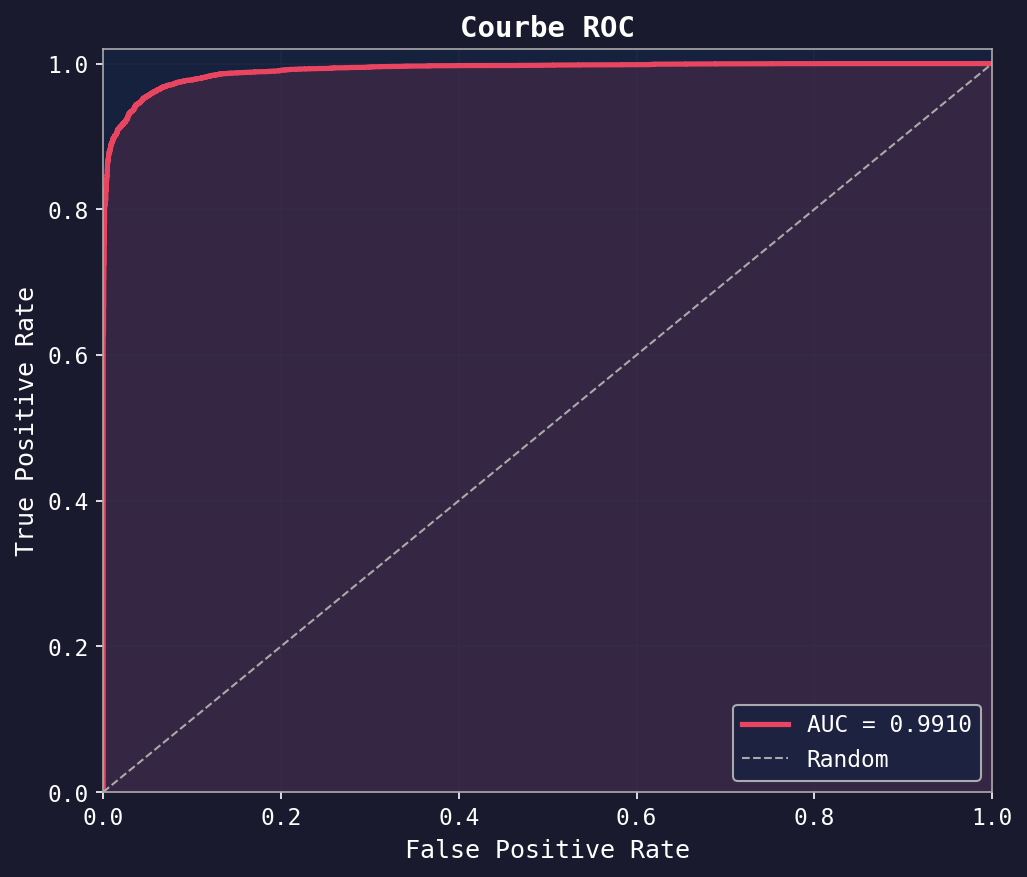
\includegraphics[width=\linewidth,
    trim=30 20 30 20,clip]{roc_curve}
\end{column}
\begin{column}{0.495\linewidth}
  \textbf{\small Precision-Recall:}\\[3pt]
  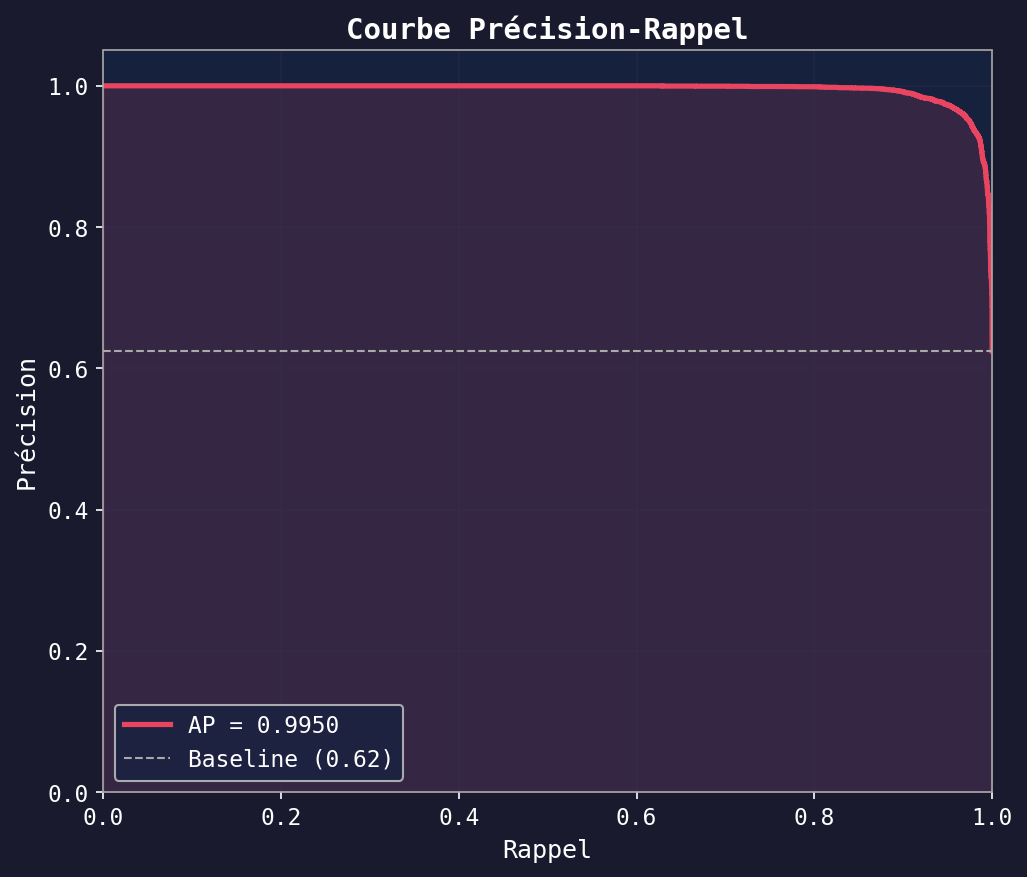
\includegraphics[width=\linewidth,
    trim=30 20 30 20,clip]{precision_recall}
\end{column}
\end{columns}

\vspace{6pt}

\begin{columns}[T]
\begin{column}{0.495\linewidth}
  \textbf{\small Score Distribution:}\\[3pt]
  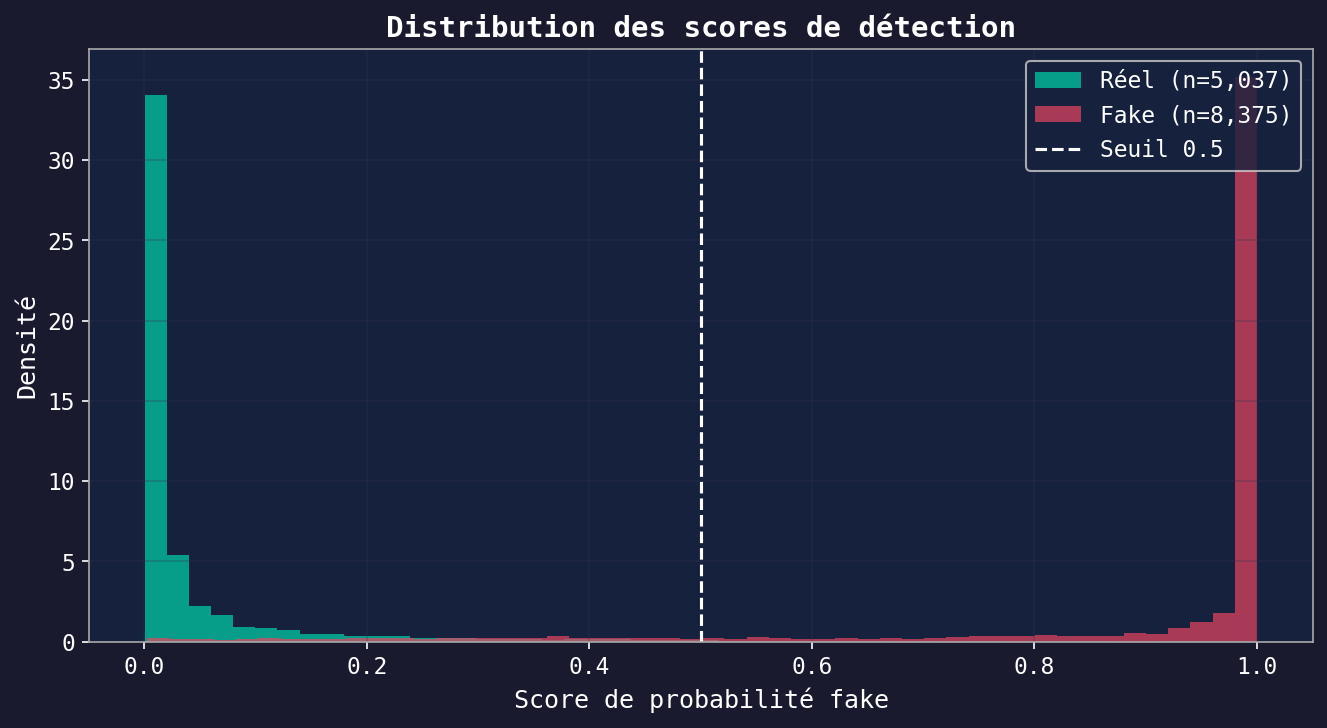
\includegraphics[width=\linewidth,
    trim=30 20 30 20,clip]{score_distribution}
\end{column}
\begin{column}{0.495\linewidth}
  \textbf{\small Training Curves:}\\[3pt]
  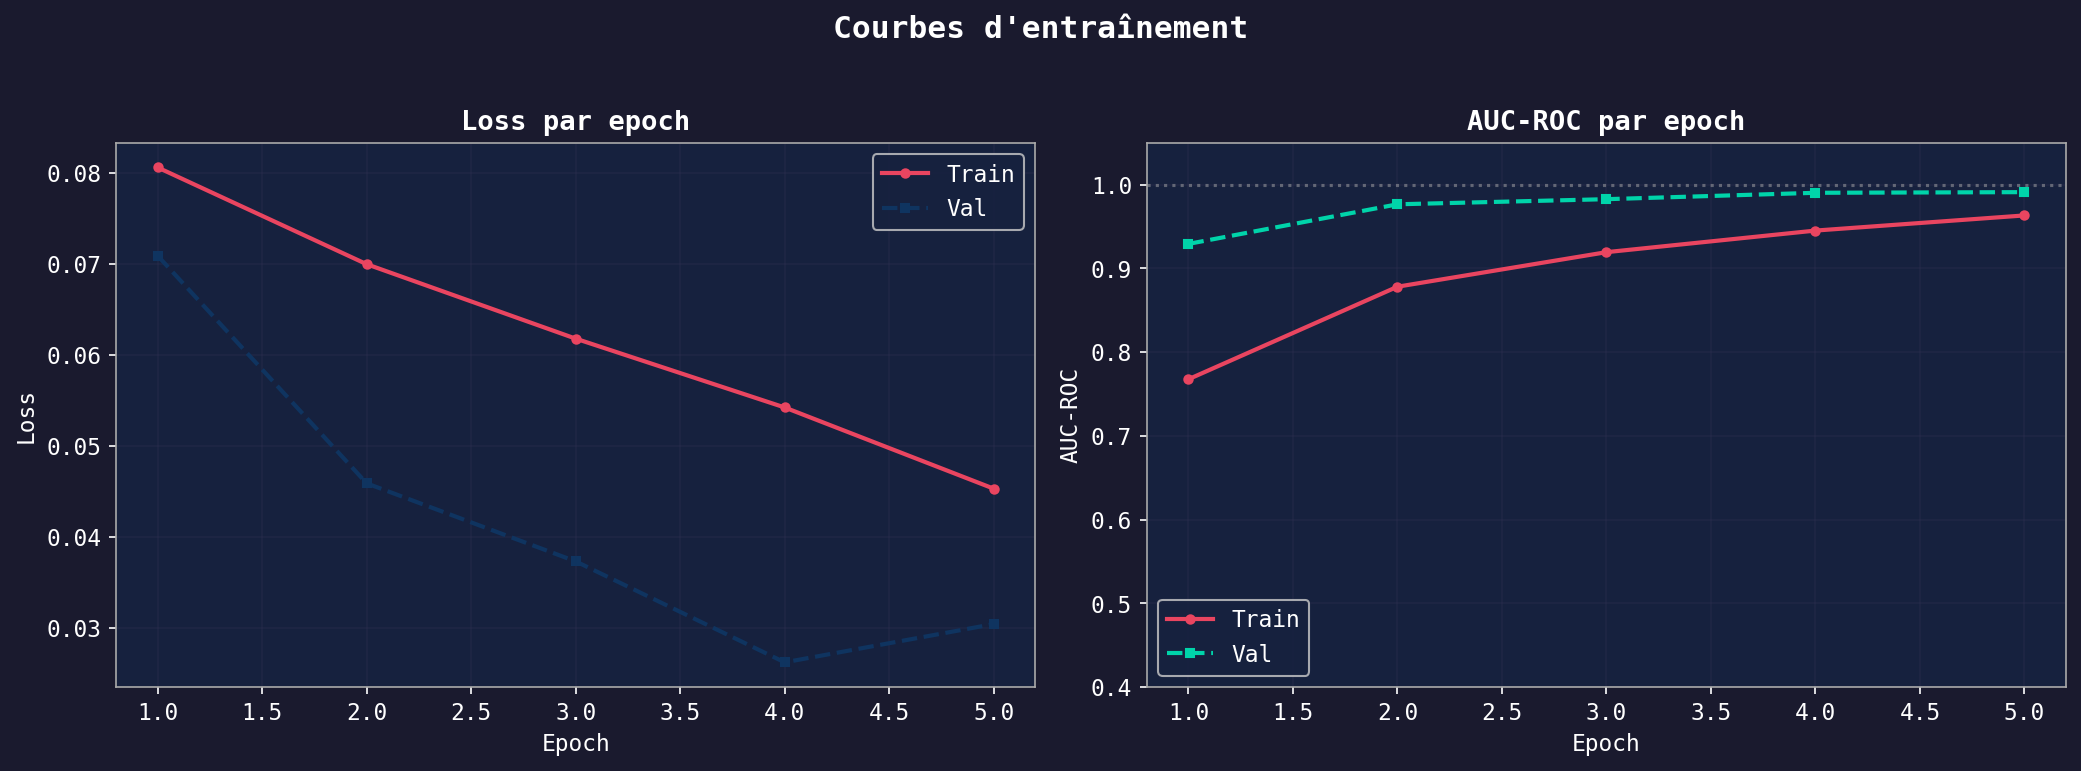
\includegraphics[width=\linewidth,
    trim=30 20 30 20,clip]{training_curves}
\end{column}
\end{columns}
\end{tcolorbox}

\end{column}

%% ─────────────────────────────────────────────────────────────
%%  COL 3  — Confusion + Calibration + Samples + Baselines + Conclusion
%% ─────────────────────────────────────────────────────────────
\begin{column}{0.295\linewidth}

%% Confusion matrix
\begin{tcolorbox}[card, title={\faTable\ \ Confusion Matrix},
  colbacktitle=Teal, coltitle=White]
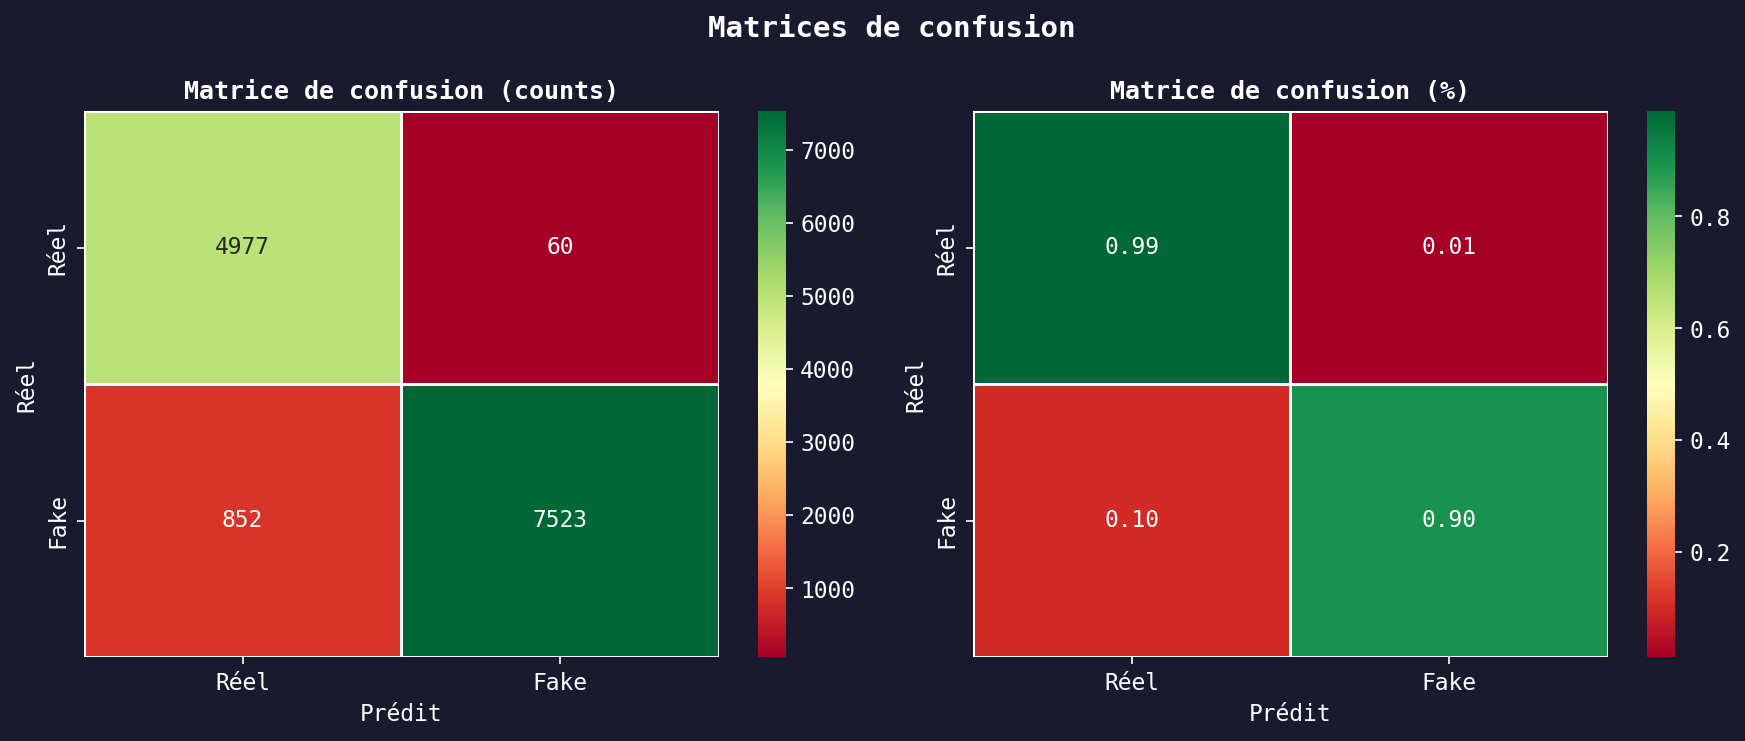
\includegraphics[width=\linewidth, trim=30 20 30 20, clip]{confusion_matrix}
\end{tcolorbox}

\vspace{8pt}

%% Calibration
\begin{tcolorbox}[card, title={\faThermometerHalf\ \ Calibration},
  colbacktitle=Amber, coltitle=Navy]
\RaggedRight\small
Single scalar $T^*$ learned via LBFGS on val set:
$\hat{p} = \sigma\!\left(\tfrac{f(x)}{T^*}\right)$

\vspace{4pt}
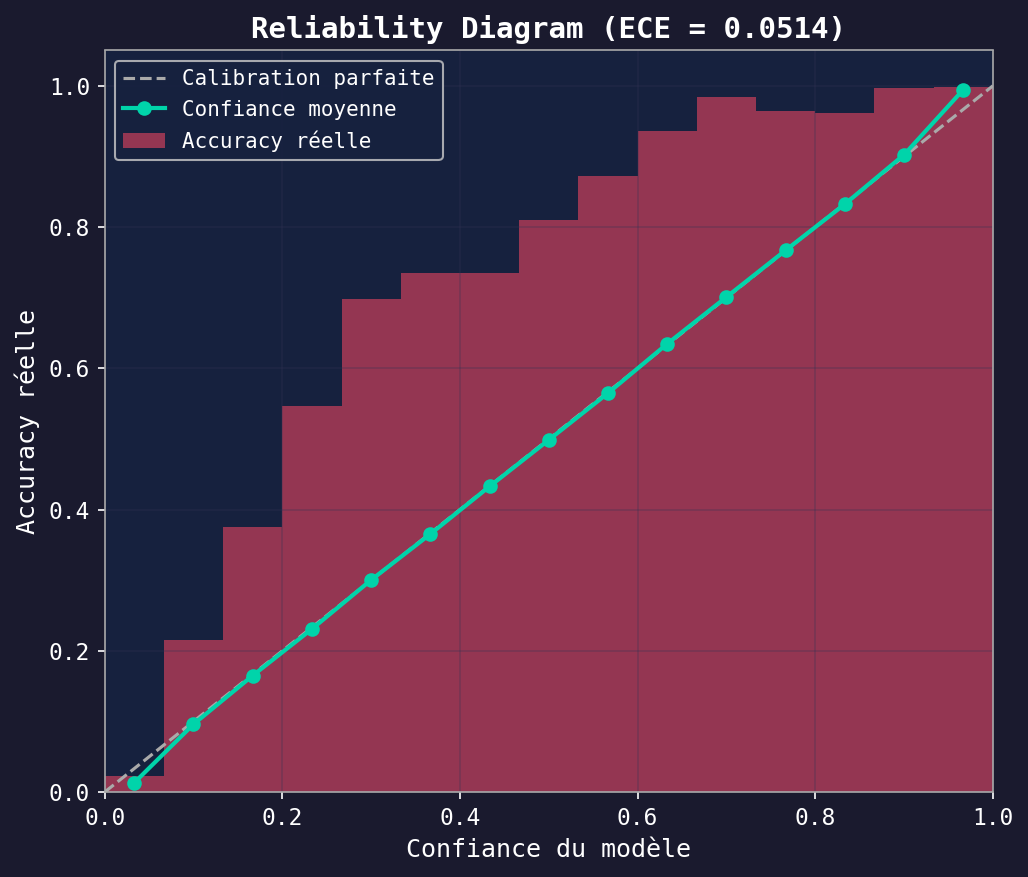
\includegraphics[width=\linewidth, trim=30 20 30 20, clip]{reliability_diagram}

\vspace{3pt}
\textbf{ECE = 0.0250} — well-calibrated
(\textit{threshold}: ECE $<$ 0.05 is good).
\end{tcolorbox}

\vspace{8pt}

%% Sample predictions
\begin{tcolorbox}[card, title={\faSearch\ \ Sample Predictions},
  colbacktitle=Navy, coltitle=White]
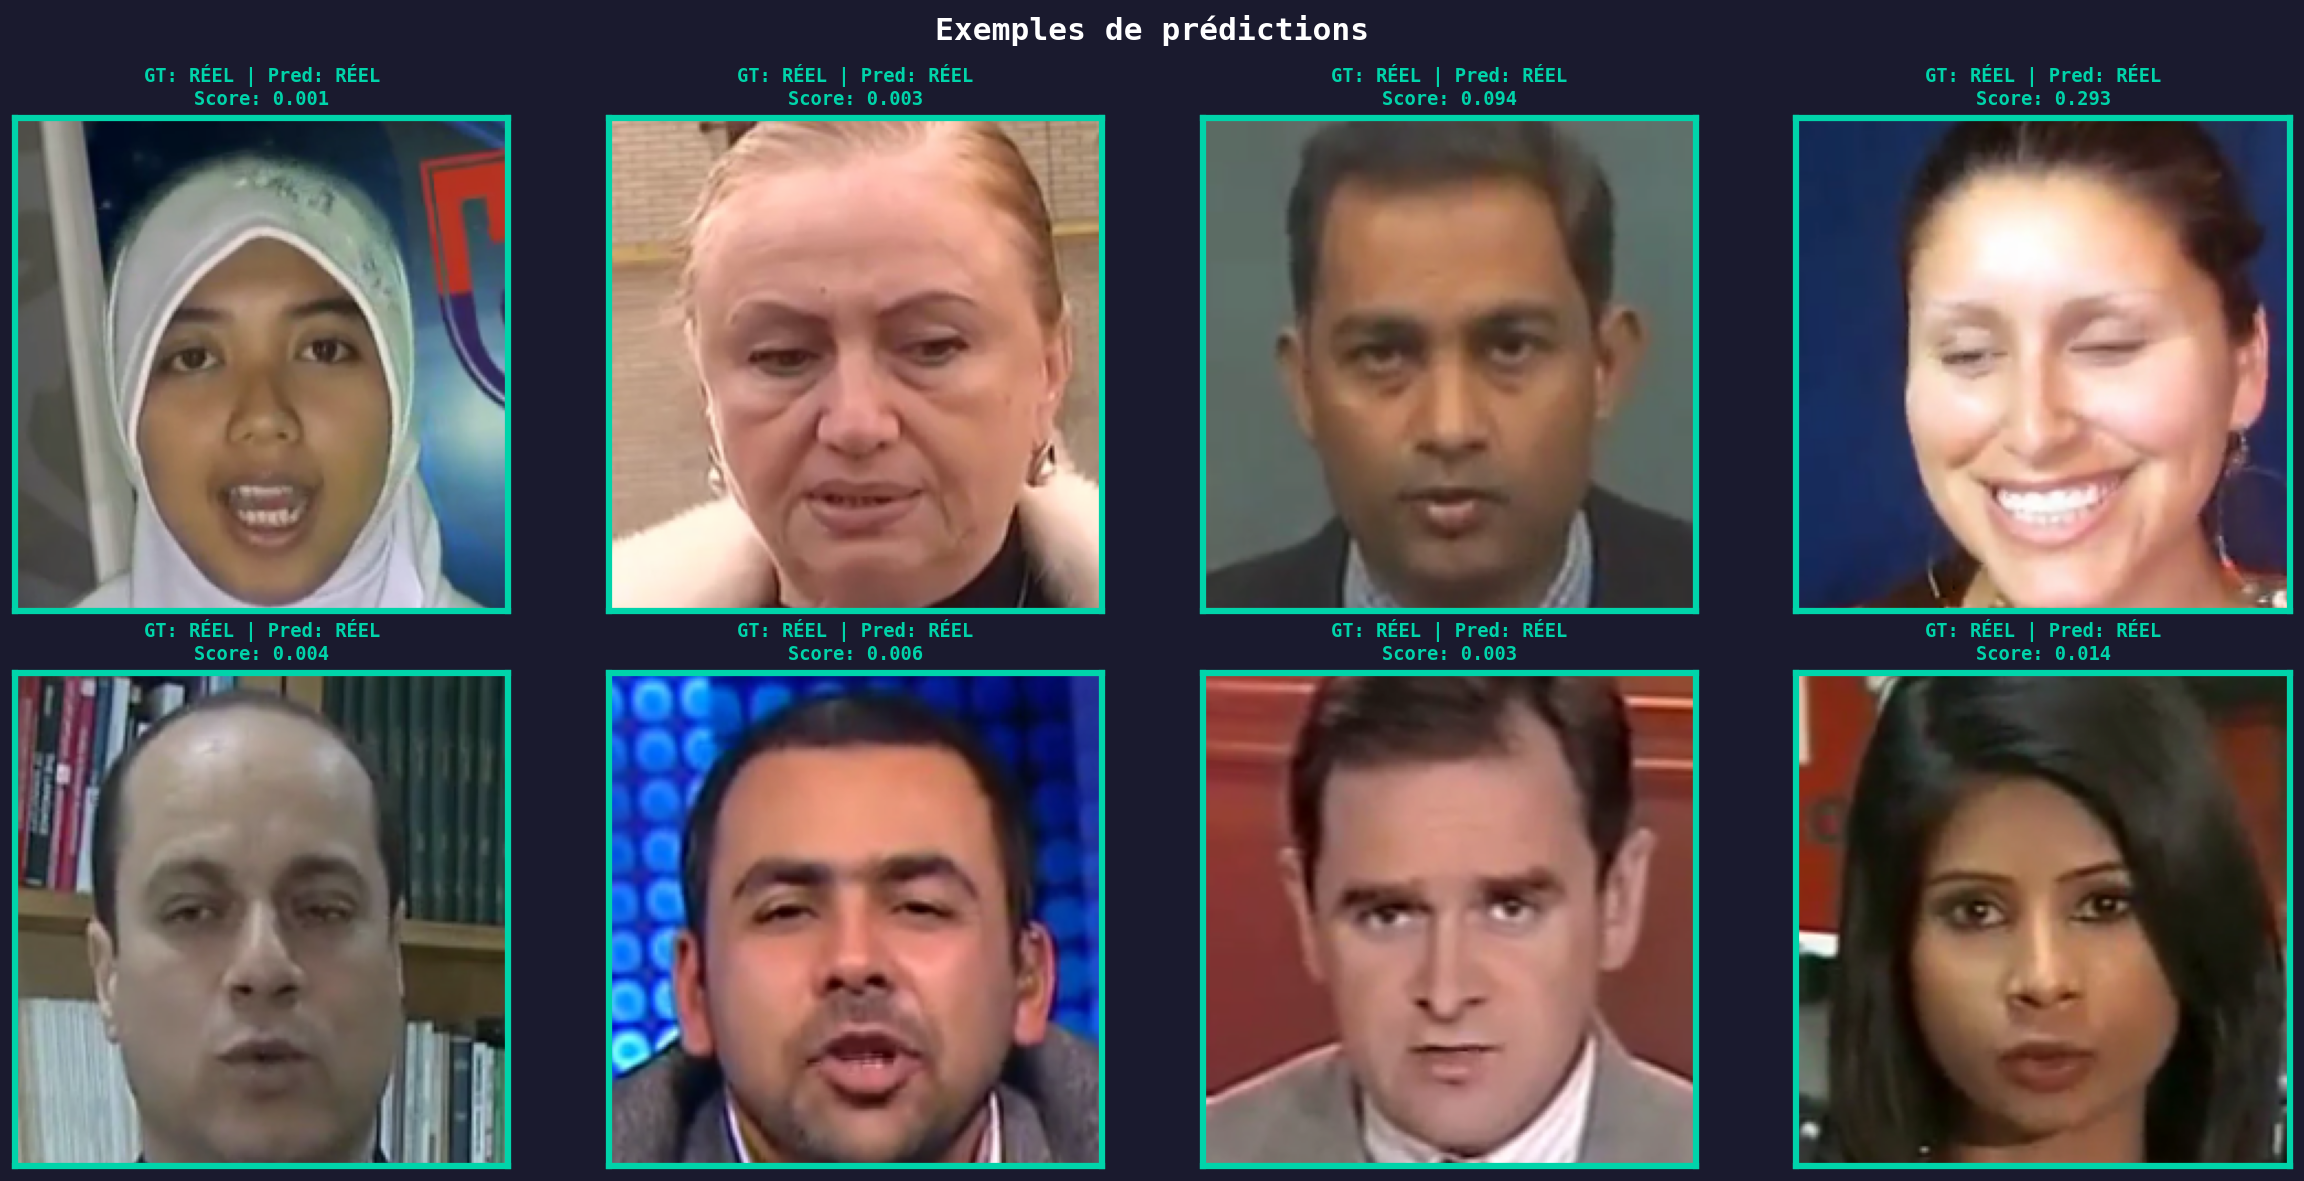
\includegraphics[width=\linewidth, trim=20 10 20 10, clip]{sample_predictions}
{\small\itshape Green border = correctly classified · Red = error.
Each image shows predicted $P(\text{fake})$.}
\end{tcolorbox}

\vspace{8pt}

%% Baseline comparison
\begin{tcolorbox}[card, title={\faBalanceScale\ \ Comparison with Baselines},
  colbacktitle=Blue, coltitle=White]
{\small\renewcommand{\arraystretch}{1.25}
\begin{tabularx}{\linewidth}{@{}>{\bfseries}l
  >{\centering}X >{\centering}X >{\centering\arraybackslash}X@{}}
\toprule
\rowcolor{Navy!10} Method & AUC & ECE & Params \\
\midrule
\rowcolor{RowA}  Xception (FF++) & 0.912 & 0.089 & 22M \\
                 EfficientNet-B4 & 0.934 & 0.071 & 19M \\
\rowcolor{RowA}  CLIP + Linear   & 0.951 & 0.062 & 86M \\
                 ResNet-50 + FFT & 0.947 & 0.058 & 25M \\
\midrule
\rowcolor{Red!15}\textbf{Ours}  & \textbf{.9898} & \textbf{.025} & \textbf{89M} \\
\bottomrule
\end{tabularx}}
{\footnotesize\itshape Baselines re-evaluated on DF40 val set.}
\end{tcolorbox}

\vspace{8pt}

%% Conclusions
\begin{tcolorbox}[card, title={\faCheckCircle\ \ Conclusions \& Future Work},
  colbacktitle=Green, coltitle=White]
\RaggedRight\small
\textbf{Key contributions:}
\begin{itemize}[leftmargin=1.3em,itemsep=2pt]
  \item[\textcolor{Green}{\faCheck}]
    Dual-branch fusion of \textbf{semantic} (DINOv2) + \textbf{spectral} (FFT/DCT)
  \item[\textcolor{Green}{\faCheck}]
    \textbf{AUC\,=\,0.9898} on 10-method DF40 subset
  \item[\textcolor{Green}{\faCheck}]
    \textbf{ECE\,=\,0.025} — reliable calibrated probabilities
  \item[\textcolor{Green}{\faCheck}]
    Generalizes across GAN, Diffusion, Reenactment \& Editing
\end{itemize}

\vspace{5pt}
\textbf{Future work:}
\begin{itemize}[leftmargin=1.3em,itemsep=2pt]
  \item[\textcolor{Amber}{\faArrowRight}]
    Test on Sora / DALL-E\,3 (proprietary, not in DF40)
  \item[\textcolor{Amber}{\faArrowRight}]
    Temporal modeling for video deepfakes
  \item[\textcolor{Amber}{\faArrowRight}]
    GradCAM explainability on spatial branch
  \item[\textcolor{Amber}{\faArrowRight}]
    Adversarial robustness study
\end{itemize}
\end{tcolorbox}

\end{column}
\end{columns}

\vspace{10pt}

%% ══════════════════════════════════════════════════════════════
%%  FOOTER
%% ══════════════════════════════════════════════════════════════
\begin{tcolorbox}[
  enhanced, arc=0pt, boxrule=0pt,
  colback=Navy, borderline north={4pt}{0pt}{Red},
  top=7pt, bottom=7pt, left=18pt, right=18pt,
]
\begin{center}
{\small\sffamily\color{White!70}
  \faCode\ \ \texttt{github.com/anessrb/Deepfakedetection}
  \quad\textbullet\quad
  \faDatabase\ \ DF40 Dataset — NeurIPS 2024
  \quad\textbullet\quad
  \faEnvelope\ \ Anes Rabhi
  \hfill
  Deep Learning for Computer Vision — 2025
}
\end{center}
\end{tcolorbox}

\end{frame}
\end{document}
